We have run two different versions of the model: one that is the same as \cite{li2018deep} in order to report on the original paper's reproducibility and another version that runs the newly proposed hierarchical version of this model. Firstly, we will discuss the replicated results of the original paper. Secondly, we will discuss the results of the hierarchical model.

\subsection{Reproduced Results}
\begin{figure}
    \centering
    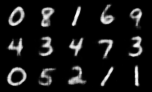
\includegraphics{img/normalprot1499.png}
    \caption{Original prototypes after 1500 epochs}
    \label{normalprots}
\end{figure}

After training our implementation of the original prototype model for 1500 epochs with 15 prototypes and a learning rate of 0.0001 as done by \cite{li2018deep} we achieved an accuracy of 98.8\%. This corroborates the results of the original paper. Moreover, it shows that the addition of a prototype layer does not significantly reduce the accuracy that the model is able to achieve. 

We pushed the 15 prototypes that our implementation of the original prototype network produced through the decoder to visualize them. These are shown in Figure~\ref{normalprots}. As in the original paper \cite{li2018deep}, the prototypes resemble authentic handwritten digits. This further confirms that we can replicate the results of the original paper, namely that we can generate meaningful and interpretable prototypes.

\subsection{Hierarchical Results}
Subsequently, we extended the architecture in the original paper \cite{li2018deep} and we implemented and trained this hierarchical prototype model. After training the hierarchical prototype model for 1500 epochs, it achieved 98.9\% accuracy and 99.0\% accuracy for the superprototype and the subprototype classification network respectively on the MNIST test set. These accuracies are nearly identical to the ones found in our implementation of the original prototype paper and to the accuracy reported in \cite{li2018deep}. This points towards our hierarchical prototype model being equally as capable of making accurate predictions on the MNIST as the other two models are. 
\begin{figure}[ht]
    \centering
    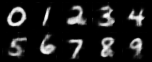
\includegraphics{img/prot1499.png}
    \caption{Superprototypes after 1500 epochs with weights set to negative identity.}
    \label{superprots}
\end{figure}

Next, by passing the learned superprototypes through the trained decoder, we visualized the learned superprototypes as shown in Figure~\ref{superprots}. By fixing the weight matrix to the negative identity matrix, we ensure that the model learns one prototype that resembles a distinct class within our data for every class \cite{li2018deep}. In case of the MNIST data set, these classes are the digits 0-9. Because of the fixed weight matrix, the superprototypes shown in Figure~\ref{superprots} each represent a different digit corresponding to our expectation. The learned superprototypes are crisp and easily interpretable representations of handwritten digits.

\begin{figure}[ht]
    \centering
    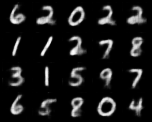
\includegraphics{img/subprot1499.png}
    \caption{20 subprototypes after 1500 epochs with learnable weights}
    \label{subprots}
\end{figure}

We trained the superprototypes simultaneously with the subprototypes in our model. Again, we visualized these subprototypes by passing their latent representations through the decoder and displayed the results as shown in Figure~\ref{subprots}. Because the weight matrix connecting the 20 neuron subprototype layer to the 10 class output layer has learnable parameters, the network itself determines how many subprototypes it gives to every class. As shown in Figure~\ref{subprots} the model finds at least one subprototype per class. 

Consequently, some interesting subprototypes show up. The model finds 4 different visualisations of a 2. One explanation is that it learns to model a number of different ways the 2 can be written, whether it is more straight or has a loop connecting the bottom part to the main diagonal. For the 1s, our model learns 3 different representations, mostly variations in how much they are tilted to the right. The variations in the 6s follow a similar pattern. Finally, some subprototypes represent mostly a specific class but can also be construed as trying to capture several digits at once and use it in their classification. For example, the 8 in the third column, fourth row can also be seen as being a hybrid between an 8 and a 9. 

P